\documentclass[11pt]{article}
\usepackage[utf8]{inputenc}
\usepackage[francais]{babel}
\usepackage{amsmath}
\usepackage{amssymb}
\usepackage{listings} 
\usepackage{color}
\usepackage[usenames,dvipsnames,svgnames,table]{xcolor}
\usepackage{colortbl}
\usepackage{hyperref}
\usepackage[a4paper]{geometry}
\usepackage{graphicx}
\usepackage{fancyhdr}
\pagestyle{fancy}
\fancyfoot[C]{\textbf{page \thepage/26}}
\fancyhead[L]{\leftmark}
\fancyhead[R]{\rightmark}
\geometry{hscale=0.75,vscale=0.80,centering}
\lstdefinestyle{customc}{
  belowcaptionskip=1\baselineskip,
  breaklines=true,
  xleftmargin=\parindent,
  language=C,
  showstringspaces=false,
  basicstyle=\footnotesize\ttfamily,
  keywordstyle=\bfseries\color{ForestGreen},
  commentstyle=\itshape\color{purple},
  identifierstyle=\color{blue!60!black},
  stringstyle=\color{orange},
}
\lstdefinestyle{customasm}{
  belowcaptionskip=1\baselineskip,
  xleftmargin=\parindent,
  language=[x86masm]Assembler,
  basicstyle=\footnotesize\ttfamily,
  commentstyle=\itshape\color{purple},
}
\lstset{escapechar=@,style=customc}
\title{Naval Batal}
\author{Jordan Barbier et Yoann Bourgery }
\date{11 Décembre 2015}

\begin{document}
\begin{titlepage}
  \begin{sffamily}
    \begin{center}
      
\includegraphics[scale=0.07]{image/enseirb-matmeca.png}\\
      \vspace{1cm}
      \textsc{\LARGE Rapport de projet 1A}\\
      \vspace{1.5cm}
      \rule{\linewidth}{.5pt}
      \vspace{0.5cm}
      \\
      {\huge \bfseries Naval Batal}
      \\
      \vspace{0.5cm}
      \rule{\linewidth}{.5pt}\\
      \vspace{0.5cm}
      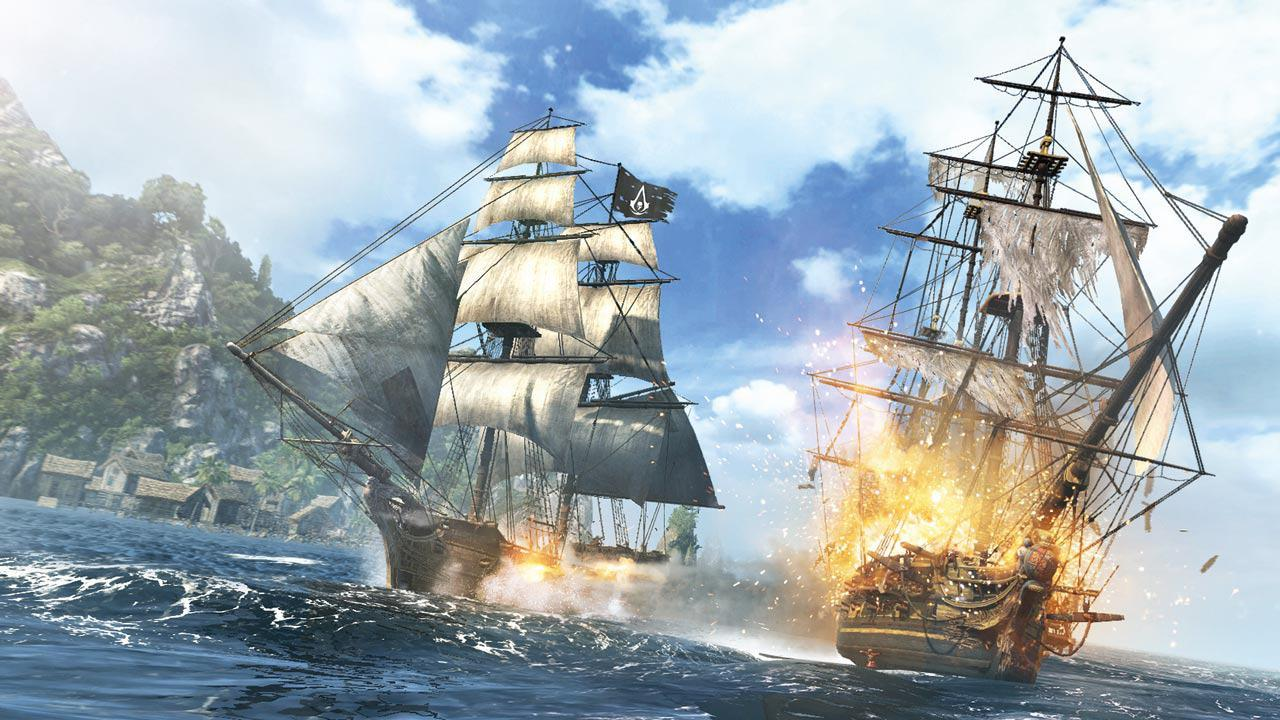
\includegraphics[scale=0.3]{image/Naval_battle.png}\\
      \vspace{0.5cm}
      \begin{minipage}{0.4\textwidth}
          \begin{flushleft}
            \begin{large}
              Barbier Jordan\\
              Bourgery Yoann\\
            \end{large}
          \end{flushleft}
        \end{minipage}
        \begin{minipage}{0.4\textwidth}
            \begin{flushright}
              \begin{large}
                {\textit Encadrant : M. Ahmed Toufik}
              \end{large}
            \end{flushright}
        \end{minipage}
        \vfill
        {\large 16 Octobre 2015 - 11 Décembre 2015}
    \end{center}
  \end{sffamily}
\end{titlepage}
\newpage
\tableofcontents
\newpage
\section{Introduction}

Le thème du projet est \textbf{Naval Batal}, le but de ce projet est donc d'implémenter le jeu Naval Batal en langage C. 

\subsection{Le principe du Jeu}

Le jeu Naval Batal est un jeu dont les règles sont inspirées d'une bataille navale classique, c'est à dire que chaque joueur possède une grille de case sur laquelle peut se situer des bateaux (appelés Batal ici) et le but du joueur est de toucher les cases des bateaux de son adversaire. Une fois toutes les cases de l'adversaire touchées, le joueur gagne la partie.

\subsection{Définition des problèmes de ce projet}

On peut soulever plusieurs problèmes à résoudre, plusieurs questions à se poser avant de commencer à coder ce projet. Les questions rencontrées sont les suivantes avec leurs solutions (solutions qui peuvent avoir été prises en début de projet puis modifier pour une meilleure implémentation) :\\
\begin{itemize}
\item \textbf{Comment implémenter la grille de chaque joueur ? Faut-il faire une grille pour chaque joueur ? Ou alors faire une grille commune pour contenir toutes les informations en même temps ?} \\
Face à cette question, nous avons opté pour une grille commune implémentée sous forme d'un tableau linéaire d'entier. Chaque case de la grille contiendrait 0 pour de l'eau, 1 pour un bateau du joueur1, 2 pour un bateau du joueur2, 3 pour un bateau du joueur1 et simultanément du joueur2 et enfin -1 pour un case oblitéré. Cette structure sera modifiée plus tard dans le projet pour un tableau linéaire contenant, non plus des entiers, mais un tableau d'entier de taille {\textit{NB\_JOUEURS}} + 1 qui en case 0 contient l'information si la case est oblitérée ou non (-1 pour oblitéré, 0 sinon) et dans les positions i appartenant à [1,{\textit{NB\_JOUEURS}}], chaque case contient 1 si le $joueur_{i}$ possède un bateau présent sur cette case, 0 sinon. L'idée étant, dans une évolution future du jeu, de pouvoir implémenter plus de deux joueurs (ce qui n'a pas été demandé par la suite).\\

\item \textbf{Comment implémenter un bateau ? Comment implémenter un joueur ?} \\
La question qui nous a traversé l'esprit étant la nécessité de faire une structure de joueur ou/et de faire une structure de bateau. Et pour une raison de simplicité de code (au niveau de la relecture et au niveau de la programmation), nous avons trouvés plus simple de créer une structure de bateau et une structure de joueur.\\

\item \textbf{Comment afficher une grille ?} \\ 
Pour une meilleure compréhension de ce que nous faisions, en plus des fonctions de test, il était nécessaire de faire un affichage clair d'une partie et nous avons donc opté pour un affichage simple en texte dans la console du terminal. C'est seulement plus tard que nous avons opté pour un affichage plus avancé avec les fonctions de SDL.\\
\end{itemize}
\begin{lstlisting}
\end{lstlisting}
\newpage
\section{Achievement0}
\subsection{Définition des constantes et macro}

L'utilisation de constante nous permet de modifier plus simplement des
éléments clefs du jeu. Pour cela nous utilisons les constantes suivantes
:  
\begin{itemize}
\item {\textit{NB\_JOUEURS}} : Nous permet de modifier le nombre de
  joueur en théorie.
\item {\textit{NB\_LIGNES}} : Nous permet de modifier le nombre de
  ligne dans la grille de notre jeu.
\item {\textit{NB\_COLONNES}} : Nous permet de modifier le nombre de
  colonne dans la grille de notre jeu.
\item {\textit{NB\_BATALS}} : Nous permet de modifier le nombre de
  bateau dans le jeu.
\item {\textit{NB\_MONSTRES}} : Nous permet de modifier le nombre de
  monstre en théorie (cf : ACHIEVEMENT3).
\item {\textit{NB\_PIXEL\_CASE}} : Nous permet de modifier la taille
  d'une case dans la représentation graphique en SDL.
\item {\textit{TAILLE\_MAX\_BAT}} : C'est la taille maximale qu'un
  bateau peut avoir, elle nous permet de pouvoir initialiser la
  structure Batal et Joueur.
\item {\textit{TAB\_TAILLE}} : Cette constante nous permet d'obtenir un tableau d'entier où chaque entier représente la taille du bateau d'indice i du tableau.
\end{itemize}
On utilise aussi une macro qui nous permet de mettre de la couleur
dans le terminal.

\subsection{Définition des structures}

\subsubsection{Position}
Cette structure nous permet de nous repérer dans la grille, elle contient : 
\begin{itemize}
\item Un entier qui correspond à la ligne
\item Un entier qui correspond à la colonne
\end{itemize}

\subsubsection{Case}

Cette structure nous permet de savoir l'état d'une position de la grille, elle contient :
\begin{itemize}
\item Un tableau d'entier où l'indice 0 correspond à une case qui
  est oblitérée ou non (-1 : oblitérée, 0 : intact) et l'indice 1 à
  {\textit{NB\_JOUEURS}} permet de savoir si un bateau du joueur est dans
  cette case (1 : présent, 0 : absent) et de même pour le monstre
  à l'indice {\textit{NB\_JOUEURS}} + 1 (1 : présent, 0 : absent)
\end{itemize}

\subsubsection{Grille}

Cette structure permet de représenter la grille du jeu, elle contient
:
\begin{itemize}
\item Un tableau de {\textit{NB\_LIGNES}} * {\textit{NB\_COLONNES}}
  Cases pour représenter entièrement notre grille.
\end{itemize}

\subsubsection{Alignement}
Cette énumération nous permet d'associer à chaque bateau une forme et/ou un alignement, par exemple savoir si le bateau est horizontal, si le bateau est vertical, si le bateau est en O, en H, ou en L dans une certaine orientation. Il faut savoir que les bateaux linéaires horizontaux ou verticaux peuvent avoir une taille quelconque tant que celle-ci ne dépasse pas le nombre de lignes de la grille pour le batal vertical ou le nombre de colonnes pour le batal horizontal. Si le bateau est en O, alors nécessairement, il aura une taille de 8, s'il est en H, il aura une taille de 7 et s'il est en L, une taille de 4. Voici un schéma associant chaque nombre de l'énumération à un type de bateau. 
\begin{flushleft}
\begin{tabular}[t]{|c|c|c|c|c|}
  \hline
  & & & &  \\
  \hline
  & & & &  \\
  \hline
  & \cellcolor{blue} & \cellcolor{blue} & \cellcolor{blue} &   \\
  \hline
  & & & &  \\
  \hline
  & & & &  \\
  \hline
  \multicolumn{5}{c}{Enum 1}\\
\end{tabular}
\hspace{3cm}
\begin{tabular}[t]{|c|c|c|c|c|}
  \hline
  & & & &  \\
  \hline
  & & \cellcolor{blue} & &  \\
  \hline
  & & \cellcolor{blue} & &  \\
  \hline
  & & \cellcolor{blue} & &  \\
  \hline
  & & & &  \\
  \hline
  \multicolumn{5}{c}{Enum 10}\\
\end{tabular}
\hspace{3cm}
\begin{tabular}[t]{|c|c|c|c|c|}
  \hline
  & & & &  \\
  \hline
  & \cellcolor{blue}& \cellcolor{blue}& \cellcolor{blue}&  \\
  \hline
  & \cellcolor{blue}& & \cellcolor{blue}&  \\
  \hline
  & \cellcolor{blue}& \cellcolor{blue}& \cellcolor{blue}&  \\
  \hline
  & & & &  \\
  \hline
  \multicolumn{5}{c}{Enum 20}\\
\end{tabular}
\end{flushleft}
\begin{flushleft}
\begin{tabular}[t]{|c|c|c|c|c|}
  \hline
  & & & &  \\
  \hline
  & \cellcolor{blue}& & \cellcolor{blue}&  \\
  \hline
  & \cellcolor{blue} &\cellcolor{blue}  & \cellcolor{blue} &   \\
  \hline
  & \cellcolor{blue}& &\cellcolor{blue} &  \\
  \hline
  & & & &  \\
  \hline
  \multicolumn{5}{c}{Enum 31}\\
\end{tabular}
\hspace{3cm}
\begin{tabular}[t]{|c|c|c|c|c|}
  \hline
  & & & &  \\
  \hline
  & \cellcolor{blue}&  \cellcolor{blue}& \cellcolor{blue}&  \\
  \hline
  & & \cellcolor{blue} & &  \\
  \hline
  &\cellcolor{blue} & \cellcolor{blue} & \cellcolor{blue} &  \\
  \hline
  & & & &  \\
  \hline
  \multicolumn{5}{c}{Enum 32}\\
\end{tabular}
\hspace{3cm}
\begin{tabular}[t]{|c|c|c|c|c|}
  \hline
  & & & &  \\
  \hline
  & \cellcolor{blue}& & &  \\
  \hline
  &  \cellcolor{blue}&  &  &   \\
  \hline
  & \cellcolor{blue}& \cellcolor{blue}& &  \\
  \hline
  & & & &  \\
  \hline
  \multicolumn{5}{c}{Enum 41}\\
\end{tabular}
\end{flushleft}
\begin{flushleft}
\begin{tabular}[t]{|c|c|c|c|c|}
  \hline
  & & & &  \\
  \hline
  & & \cellcolor{blue}& &  \\
  \hline
  & &  \cellcolor{blue}&  &   \\
  \hline
  & \cellcolor{blue}& \cellcolor{blue}& &  \\
  \hline
  & & & &  \\
  \hline
  \multicolumn{5}{c}{Enum 42}\\
\end{tabular}
\hspace{3cm}
\begin{tabular}[t]{|c|c|c|c|c|}
  \hline
  & & & &  \\
  \hline
  & \cellcolor{blue}&  \cellcolor{blue}& &  \\
  \hline
  & \cellcolor{blue}&  & &  \\
  \hline
  & \cellcolor{blue}&  & &  \\
  \hline
  & & & &  \\
  \hline
  \multicolumn{5}{c}{Enum 43}\\
\end{tabular}
\hspace{3cm}
\begin{tabular}[t]{|c|c|c|c|c|}
  \hline
  & & & &  \\
  \hline
  & \cellcolor{blue}& \cellcolor{blue} & &  \\
  \hline
  & & \cellcolor{blue} & &  \\
  \hline
  & &  \cellcolor{blue}& &  \\
  \hline
  & & & &  \\
  \hline
  \multicolumn{5}{c}{Enum 44}\\
\end{tabular}
\end{flushleft}
\begin{flushleft}
\begin{tabular}[t]{|c|c|c|c|c|}
  \hline
  & & & &  \\
  \hline
  & & & \cellcolor{blue}&  \\
  \hline
  & \cellcolor{blue} &  \cellcolor{blue}& \cellcolor{blue} &   \\
  \hline
  & & & &  \\
  \hline
  & & & &  \\
  \hline
  \multicolumn{5}{c}{Enum 45}\\
\end{tabular}
\hspace{3cm}
\begin{tabular}[t]{|c|c|c|c|c|}
  \hline
  & & & &  \\
  \hline
  &\cellcolor{blue} & \cellcolor{blue} &\cellcolor{blue} &  \\
  \hline
  & &  &\cellcolor{blue} &  \\
  \hline
  & &  & &  \\
  \hline
  & & & &  \\
  \hline
  \multicolumn{5}{c}{Enum 46}\\
\end{tabular}
\hspace{3cm}
\begin{tabular}[t]{|c|c|c|c|c|}
  \hline
  & & & &  \\
  \hline
  & \cellcolor{blue}&  & &  \\
  \hline
  & \cellcolor{blue}&\cellcolor{blue} &\cellcolor{blue} &  \\
  \hline
  & &  & &  \\
  \hline
  & & & &  \\
  \hline
  \multicolumn{5}{c}{Enum 47}\\
\end{tabular}
\end{flushleft}
\hspace{5.32cm}
  \begin{tabular}[t]{|c|c|c|c|c|}
  \hline
  & & & &  \\
  \hline
  & \cellcolor{blue}&\cellcolor{blue} &\cellcolor{blue} &  \\
  \hline
  & \cellcolor{blue}&  & &  \\
  \hline
  & &  & &  \\
  \hline
  & & & &  \\
  \hline
  \multicolumn{5}{c}{Enum 48}\\
  \end{tabular}
\subsubsection{Batal}

Cette structure nous permet de représenter un bateau dans le jeu, elle
contient :
\begin{itemize}
\item Un entier qui représente la taille du bateau
\item Un tableau de Position correspondant à toutes les positions
  que le bateau occupe
\item Un entier qui représente l'alignement 
\item Un entier qui représente à quelle joueur appartient le bateau
\end{itemize}

\subsubsection{Joueur}

Cette structure nous permet de rassembler toutes les informations
concernant un joueur, elle contient :
\begin{itemize}
\item Un entier qui représente le numéro du joueur
\item Un tableau de Batal
\item Un tableau de Position correspondant à toutes les cases des
  bateaux qui ne sont pas encore oblitérées
\item Un entier qui correspond au nombre de Position qui sont encore
  en vie (taille courante du tableau précédent).
\end{itemize}

\subsection{Fonctionnement achievement0}

\subsubsection{Fonctions et Complexité}

\begin{itemize}

\item Les fonctions commençant par init:
\begin{lstlisting} 
void init_grille(struct Grille *grille)
void init_batal(struct Batal *joueur, int taille, struct Position *positon, int alignement, int nbjoueur)
void init_rond(struct Batal *bateau, struct Position *posinit)
void init_H(struct Batal *bateau,struct Position *posinit,int alignement)
void init_L(struct Batal *bateau,struct Position *posinit,int alignement)
void init_joueur(struct Joueur *joueur, int nbjoueur)
\end{lstlisting}
Ces fonctions vont permettre d'initialiser les différents éléments nécessaire au jeu et à la baseline. \textit{init\_grille} est de complexité linéaire en $\Theta(n)$ avec n le nombre de case de la grille. De même, \textit{init\_batal} est de complexité linéaire en $\Theta(n)$ avec n la taille du bateau initialisé.\\

\item Les fonctions \textit{placer\_batal} et \textit{verif\_pour\_mettre\_bateau}:
\begin{lstlisting} 
int verif_pour_mettre_bateau(struct Grille *grille, struct Batal *bateau)
void placer_batal(struct Grille *grille, struct Batal *bateau)
\end{lstlisting}
Ces deux fonctions permettent de placer un bateau et d'être sur que le bateau se situe bien dans la grille, dans de bonnes positions. Le principe est simple, on choisit aléatoirement une position initiale et une forme à l'aide des fonctions \textit{position\_aléatoire} et \textit{alignement\_aléatoire} et à partir de cette première case, la fonction \textit{placer\_batal} va placer le bateau si la fonction \textit{verif\_pour\_mettre\_bateau} retourne 1 pour dire que c'est possible, sinon on recommence le processus.\\
La fonction \textit{verif\_pour\_mettre\_bateau} est de complexité $\Theta(n)$ où n est la taille du bateau à vérifier.\\
\item Les fonctions pour afficher:\\
Deux affichages sont possibles pour la grille de jeu:
\begin{itemize}
\item Un affichage en texte dans la fenêtre du terminal avec la fonction \textit{afficher\_grille}, voici un exemple en image:\\
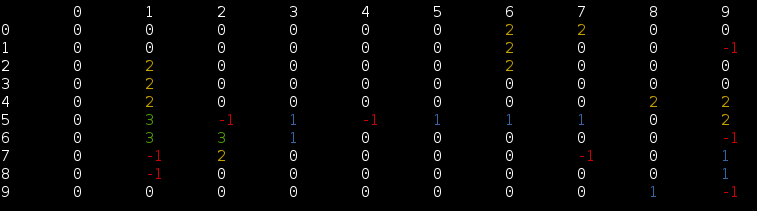
\includegraphics[scale=0.7]{image/grille_console.png}

La légende est la suivante:

\begin{itemize}
\item Le chiffre \textcolor{red}{-1} correspond à une case oblitérée.
\item Le chiffre 0 correspond à une case vide et non oblitérée.
\item Le chiffre \textcolor{blue}{1} correspond à une case occupée par un batal du joueur 1.
\item Le chiffre \textcolor{orange}{2} correspond à une case occupée par un batal du joueur 2.
\item Le chiffre \textcolor{ForestGreen}{3} correspond à une case occupée simultanément par un batal du joueur 1 et par un batal du joueur 2.
\end{itemize}

\item Un affichage en SDL dans une nouvelle fenêtre avec la fonction \textit{afficher\_grille\_SDL}, voici un exemple en image:\\

\begin{center}
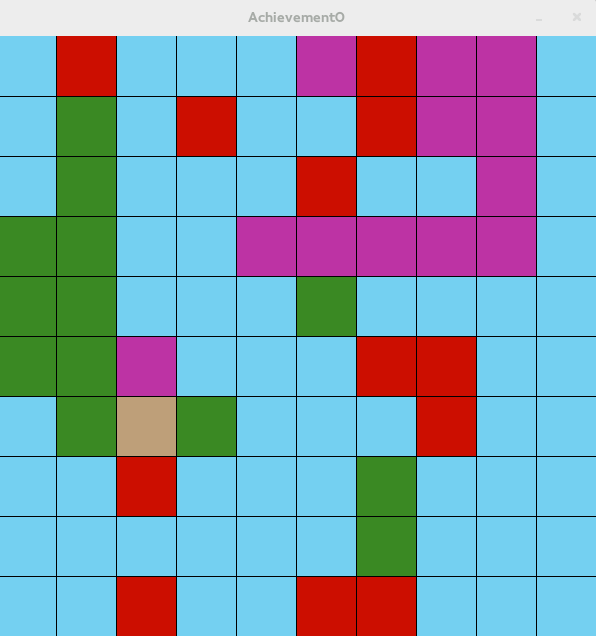
\includegraphics[scale=0.6]{image/grille_SDL.png}
\end{center}

La légende est la suivante:

\begin{itemize}
\item Les cases \textcolor{SkyBlue}{bleues} correspondent à des cases vides et non oblitérées.
\item Les cases \textcolor{red}{rouges} correspondent à des cases oblitérées.
\item Les cases \textcolor{ForestGreen}{vertes} correspondent à des cases occupées par un batal du joueur 1.
\item Les cases \textcolor{Mulberry}{violettes} correspondent à des cases occupées par un batal du joueur 2.
\item Les cases \textcolor{Tan}{beige} correspondent à des cases occupées simultanément par un batal du joueur 1 et par un batal du joueur 2.
\end{itemize}

\end{itemize}
La complexité pour les fonctions d'affichage sont de complexité linéaire en $\Theta(n)$, avec n le nombre de cases de la grille.


\item Les fonctions aléatoires:
\begin{lstlisting} 
void melange_tab();
struct Position position_aleatoire()
int alignement_aleatoire(int taille)
\end{lstlisting}
Ces trois fonctions utilisent la fonction \textit{rand} pour ainsi respectivement mélanger le tableau des positions pour obtenir ainsi plus rapidement des positions aléatoires pour une partie, retourner une position aléatoire, retourner un alignement aléatoire.

\end{itemize}

\subsubsection{Fonctionnement global du jeu}
\begin{lstlisting}
  init_grille(&grille);
  init_joueur(&joueur1, 1);
  init_joueur(&joueur2, 2);
  init_tab();
  melange_tab();
  placer_batal_joueur(&joueur1, &grille);
  placer_batal_joueur(&joueur2, &grille);
  afficher(&grille, ecran, 1, affichage);
  while(un_bateau_toujours_en_vie(&grille, &joueur1) && un_bateau_toujours_en_vie(&grille, &joueur2)){
    pos = TAB_POSITION[indice];
    obliterer_une_case(&grille, &pos, &joueur1, &joueur2);
    indice ++;
    pos = TAB_POSITION[indice];
    obliterer_une_case(&grille, &pos, &joueur1, &joueur2);
    indice ++;
    afficher(&grille, ecran, 1, affichage);
  }
  if(un_bateau_toujours_en_vie(&grille, &joueur1)){
    return(1);
    }
  if(un_bateau_toujours_en_vie(&grille, &joueur2)){
    return(2);
  }
  return(0);
\end{lstlisting}
Voici le code C permettant de simuler une partie, tout d'abord on initialise toutes nos structures utiles à la partie: 2 joueurs, la grille. Ensuite, on relie les deux grâce à la fonction \textit{placer\_batal\_joueur} qui va en même temps initialiser nos bateaux pour les deux joueurs en les plaçant à des positions possibles. Pour finir l'initialisation, on affiche pour la première fois la grille. C'est à partir de la boucle \textbf{while} que commence la partie, la fonction \textit{un\_bateau\_toujours\_en\_vie} va savoir si les joueurs sont encore en jeu (avec une case de leurs bateaux non oblitérées) ou non (toutes leurs cases oblitérées), d'où l'utilisation de cette fonction comme condition pour la boucle \textbf{while}. Ensuite, on prend, les unes après les autres, les cases du tableau de positions mélanger initialement et chaque joueur oblitère une case avec la fonction \textit{obliterer\_une\_case}. \\
On peut justifier que la boucle se termine:\\
Posons $N=NB\_COLONNES*NB\_LIGNES$ et $i=indice$, on a donc pour variant de boucle $N-i$ puisqu'une fois que toutes cases sont parcourues (dans le pire des cas), obligatoirement il n'y a plus de joueurs en jeu.\\

\subsection{Problèmes rencontrés}
Nous avons rencontrés 2 problèmes dans ce premier achievement qui sont les suivants:\\
\begin{itemize}
\item Un problème avec la fonction \textit{rand} puisqu'à chaque fois sa valeur valait la même chose. On a donc inclus en plus de la bibliothèque \textit{stdlib.h}, la bibliothèque \textit{time.h} qui permet à partir de la fonction \textit{srand} d'initialiser la fonction \textit{rand}. De plus, nous avons fait une fonction \textit{init\_rand} qui initialise avec l'appel de \textit{srand} la fonction \textit{rand} et ainsi on a donc un moyen d'obtenir un nombre aléatoire beaucoup plus efficace qu'avec la fonction \textit{rand} seulement. De même, si nous utilisons un tableau de positions que nous mélangeons au départ c'est pour un gain de temps car il n'est pas possible de retomber plusieurs fois de suite sur la même position avec cette technique.\\

\item Le deuxième problème a été de se projeter dans les futurs étapes (achievements) du projet, imaginer la mise en place de bateau en O, H ou L directement dans cet achievement, la possibilité de changer la taille des bateaux, de changer le nombre de bateaux. Nous avons donc, dans le but d'un gain d'efficacité pour les achievements suivants, essayé de mettre en place des structures et des stratégies pour gérer les futurs requêtes du jeu. 
\end{itemize}



\newpage
\section{Achievement1}
\subsection{Principe de l'achievement1}
Le but de cet achievement est de ne plus lancer des missiles aléatoires mais de calculer la distance de la cible la plus proche d'un bateau. C'est à dire on doit chercher la case adverse la plus proche en partant d'une case de notre bateau sans dépasser une certaine distance. Dans cet achievement on va considérer que notre torpille peut passer sur des cases où sont présent des bateaux alliés ou adverses.\\
Pour réaliser ceci il va nous falloir calculer toutes les distances de notre position aux positions adverses.
\subsection{Fonctionnement de l'achievement1}
Pour cet achievement on a du rajouter à notre structure Joueur un tableau de position contenant toutes les cases des bateaux qui sont toujours en vie ainsi qu'un entier qui est le nombre de case qui sont toujours en vie. De plus on a du modifier notre fonction oblitérer une case pour mettre la position qui vient d'être oblitérée à la fin du tableau qui liste les cases en vie ainsi que réduire la taille de 1.\\
De plus, on a créer deux constantes qui sont :
\begin{itemize}
\item {\textit{NB\_COUP\_MAX}} qui nous dit le nombre maximum de tour de boucle que notre programme va réaliser.
\item {\textit{PORTEE\_MAX\_TORPILLE}} qui est la distance maximale qu'une torpille peut faire.
\end{itemize}
Pour réaliser cet achievement on va avoir besoin d'une fonction qui exprime la distance entre deux cases et ainsi qu'une fonction qui nous renvoi la position la plus proche de notre position de départ.
\subsubsection{Distance minimale}
Notre fonction de distance minimale a pour prototype :
\begin{lstlisting}
int distance_minimale(struct Position *position1, struct Position *position2);
\end{lstlisting}
Cette fonction applique juste la formule $|p1.ligne - p2.ligne| + |p1.colonne - p2.colonne|$. Ce qui nous permet d'avoir la distance minimale entre deux positions. Cette fonction a pour complexité $\Theta(1)$.
\subsubsection{Arrivée de la torpille}
Cette fonction va rechercher la position la plus proche dans les cases en vie de l'adversaire sans dépasser la distance {\textit{PORTEE\_MAX\_TORPILLE}}. Cette fonction a pour prototype :
\begin{lstlisting}
int arrive_torpille(struct Position *pos_de_depart, struct Joueur *joueur, struct Position *pos_arrive);
\end{lstlisting}
Cette fonction change la position pos\_arrive par la nouvelle position ({\textit{NB\_LIGNES}} et {\textit{NB\_COLONNES}} si ce n'est pas possible). Et nous renvoi un entier qui est la distance parcourue. Cette fonction a pour complexité $\Theta(n)$ où n est le nombre de case en vie du joueur adverse.\\
\subsubsection{Affichage des torpilles}
Cette fonction affiche sur une grille à part le chemin des torpilles avec des flèches pour afficher la direction de la torpille. La "x" est le point de départ et la tête de mort est le point d'arrivé. Ce qui donne sur l'exemple suivant avec un départ en position (2, 0) et une arrivée en (9, 8):\\
\begin{center}
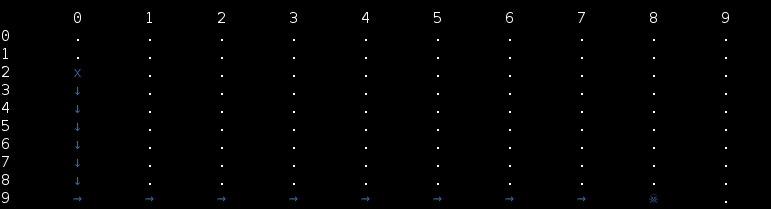
\includegraphics[scale=0.75]{./image/chemin_torpille.png}\\
\end{center}
En SDL on va avoir le chemin des torpilles de la même couleur que le joueur en un peu plus foncé.\\
Pour avoir le chemin, on va partir de la position de départ afin d'aller jusqu'à la position d'arrivée. Premièrement on va diminuer ou augmenter l'indice de ligne de la position de départ pour arriver au même que la position d'arrivée puis on va faire la même chose avec les colonnes.\\
La complexité pour afficher le chemin des torpilles est en $\Theta(n)$ où n est la distance parcourue par la torpille.
\subsubsection{Fonctionnement de la boucle de jeu}
Notre fonction qui fait tourner la boucle de jeu a pour prototype :
\begin{lstlisting}
int achievement1(SDL_Surface *ecran, int affichage);
\end{lstlisting}
Elle prend un paramètre un écran si on utilise l'affichage SDL et un entier qui permet de savoir l'affichage souhaité et retourne un entier afin de nous dire le joueur qui a gagné.\\
Notre boucle de jeu tourne tant qu'il reste des bateaux des 2 joueurs et que le nombre de coup n'a pas dépassé la constante {\textit{NB\_COUP\_MAX}}. Dans notre boucle, on va :
\begin{itemize}
\item Calculer la position d'arrivée des torpilles pour les deux joueurs.
\item Oblitérer les cases si la position d'arrivée est possible (ie ne dépasse pas la distance maximale)
\item Incrémenter le nombre de coup qui est la variable nb\_coup 
\end{itemize}
\begin{lstlisting}
  int nb_coup = 0;
  while((joueur1.taille > 0) && (joueur2.taille > 0) && (nb_coup < NB_COUP_MAX)){
    depart1 = depart_torpille(&joueur1); //On cherche le premier depart
    arrive_torpille(&(joueur1.case_en_vie[depart1]), &joueur2, &pos1); //Et arrive
    depart2 = depart_torpille(&joueur2); //On cherche le deuxieme depart
    arrive_torpille(&(joueur2.case_en_vie[depart2]), &joueur1, &pos2); // Et arrive
    if((pos1.ligne != NB_LIGNES) && (pos1.colonne != NB_COLONNES)){//Toucher
      afficher_chem(ecran, joueur1.case_en_vie[depart1], pos1, 1, grille, affichage);
      obliterer_une_case(&grille, &pos2, &joueur1, &joueur2);
      
    }
    if(affichage == 1){
      afficher_grille_SDL(&grille, ecran, 0);
      SDL_Delay(750);
    }
    if((pos2.ligne != NB_LIGNES) && (pos2.colonne != NB_COLONNES)){//Toucher
      afficher_chem(ecran, joueur2.case_en_vie[depart2], pos2, 2, grille, affichage);
       obliterer_une_case(&grille, &pos2, &joueur1, &joueur2);
    }
    nb_coup ++;
    afficher(&grille, ecran, 1, affichage);
  }
\end{lstlisting}
Notre boucle de jeu s'arrête dans tous les cas car on a l'entier n = ({\textit{NB\_COUP\_MAX}} - nb\_coup) est strictement décroissant et appartient à $\mathbb{N}$. Elle peut s'arrêter avant si le nombre de case en vie d'un joueur est nulle. 
\subsection{Problèmes rencontrés}
\begin{itemize}
\item Au début on avait oublier la possibilité qu'une torpille peut oblitérer la case des 2 joueurs, donc il a fallu modifier ça dans notre code.\\
\item Le changement de la structure Joueur nous a obligé à changer notre code dans l'achievement0 afin de pouvoir prendre en compte cette modification.
\end{itemize}

\newpage
\section{Achievement2}
\subsection{Principe de l'achievement2}
Le but de l'achievement2 est de pouvoir déplacer les bateaux à chaque tour de jeu sans que ceux-ci ne passent sur des cases qui sont oblitérées ou bien occupées par un bateau. \\
Pour réaliser cela il faut lister toutes les cases disponibles où le bateau peut aller avec une suite de translation finie.

\subsection{Fonctionnement de l'achievement2}
La fonction permettant de lister les cases possibles (ie la position de départ pour le bateau est possible) est une fonction récursive qui est appelé par une autre fonction. Son prototype est : 
\begin{lstlisting}
void liste_case_possibles(struct Grille grille, struct Batal bat, int tab[], int liste_indice_oblitere[], int tab_prec[]);
\end{lstlisting}
Cette fonction permet d'enlever le bateau dans la grille ainsi que de mettre les indices du bateau qui sont oblitérés dans le tableau liste\_indice\_oblitere (0 : oblitéré, 1 : intact), puis de lancer la fonction récursive dans les 4 directions si possible.\\
Puis ensuite il va falloir mettre à jour la grille ainsi que le bateau avec ses nouvelles positions puis le joueur afin de changer les positions de ses cases toujours en vie ainsi qu'afficher le chemin du bateau (en SDL).

\subsubsection{Principe de la fonction récursive}
Son prototype est :
\begin{lstlisting}
void liste_case_possiblesrec(struct Grille grille, struct Batal bateau, int tab[], int indice, int liste_indice_oblitere[ ], int tab_prec[ ]);
\end{lstlisting}
Cette fonction explore les cases dans les 4 directions possibles sans sortir de la grille et s'arrete lorsqu'une case est impossible ou que la case a déjà été exploré. Elle modifie le tableau tab en mettant 0 si la case n'a pas été exploré -1 si la case est impossible pour mettre le bateau et 1 si c'est possible. Le tableau tab\_prec permet de se rappeler à partir de quelle case on a pu arriver à l'indice i. Cette fonction s'arrete lorsque toutes les cases sont explorées ou lorsqu'après les 4 appels récursifs aucune case supplémentaire n'est possible (ie les cases autour sont déjà explorées ou on arrive sur une case impossible).\\
La fonction fait appel à une autre fonction qui permet de vérifier si un bateau peut se placer à cet endroit, le prototype de cette fonction est :
\begin{lstlisting}
int verif_arrive_bateau(struct Grille grille, struct Batal bat, int liste_indice_oblitere[]);
\end{lstlisting}
Cette fonction vérifie pour toute les cases du bateau toujours en vie si elle ne se trouve pas sur une case oblitérée, occupée par un monstre, un archipal ou un bateau d'un autre joueur et ne dépasse pas de la grille. Elle est de compléxitée $\Theta(m)$ où m est la taille du bateau. \\
La compléxité de la fonction récursive est donc en $\Theta(n*m)$ où n est le nombre de case de la grille. \\
Voilà un exemple de la fonction et des cases qu'elles explorent on prend la case bleu comme case de départ et les cases rouges comme oblitérées, on prend un bateau de taille 1 pour faciliter l'exemple:
\\
\begin{center}
\begin{tabular}{c|c|c|c|c|}
\multicolumn{1}{c}{} & \multicolumn{1}{c}{1} & \multicolumn{1}{c}{2} & \multicolumn{1}{c}{3} & \multicolumn{1}{c}{4}\\
\cline{2-5} 1 & 0 & \cellcolor{red}0 & 0 & 0\\
\cline{2-5} 2 & \cellcolor{red}0 & 0 & 0 & \cellcolor{red}0\\
\cline{2-5} 3 & 0 & 0 & \cellcolor{blue}0 & 0\\
\cline{2-5} 4 & 0 & 0 & 0 & 0\\
\cline{2-5}
\end{tabular}
\end{center}
On va lancer des appels récursifs sur les 4 cases autour de la case bleu, ceci se passe dans la fonction non récursive.\\
\begin{center}
\begin{tabular}{c|c|c|c|c|}
\multicolumn{1}{c}{} & \multicolumn{1}{c}{1} & \multicolumn{1}{c}{2} & \multicolumn{1}{c}{3} & \multicolumn{1}{c}{4}\\
\cline{2-5} 1 & 0 & \cellcolor{red}0 & 0 & 0\\
\cline{2-5} 2 & \cellcolor{red}0 & 0 & \cellcolor{green}0 & \cellcolor{red}0\\
\cline{2-5} 3 & 0 & \cellcolor{green}0 & 0 & \cellcolor{green}0\\
\cline{2-5} 4 & 0 & 0 & \cellcolor{green}0 & 0\\
\cline{2-5}
\end{tabular}
\end{center}
On va lancer des appels récursifs autour des 4 cases vertes car les 4 sont possibles elles vont donc prendre la valeur de 1.\\
\begin{center}
\begin{tabular}{c|c|c|c|c|}
\multicolumn{1}{c}{} & \multicolumn{1}{c}{1} & \multicolumn{1}{c}{2} & \multicolumn{1}{c}{3} & \multicolumn{1}{c}{4}\\
\cline{2-5} 1 & 0 & \cellcolor{red}0 & \cellcolor{green}0 & 0\\
\cline{2-5} 2 & \cellcolor{red}0 & \cellcolor{green}0 & 1 & \cellcolor{red}\color{blue}{0}\\
\cline{2-5} 3 & \cellcolor{green}0 & 1 & \cellcolor{green}0 & 1\\
\cline{2-5} 4 & 0 & \cellcolor{green}0 & 1 & \cellcolor{green}0\\
\cline{2-5}
\end{tabular}
\end{center}
On va lancer maintenant des appels dans les 4 directions si on ne sort pas de grille par exemple pour le 1 en position (4, 3), on ne va pas lancer d'appel récursif vers le bas car sinon on sortirait de la grille. La position (2, 4) n'est pas possible car on se trouve sur une case oblitérée on va donc mettre un -1 dans la case et ne pas lancer d'autres appels récursifs partant de cette case.\\ 
\begin{center}
\begin{tabular}{c|c|c|c|c|}
\multicolumn{1}{c}{} & \multicolumn{1}{c}{1} & \multicolumn{1}{c}{2} & \multicolumn{1}{c}{3} & \multicolumn{1}{c}{4}\\
\cline{2-5} 1 & 0 & \cellcolor{red}\color{blue}{0} & 1 & \cellcolor{green}0\\
\cline{2-5} 2 & \cellcolor{red}\color{blue}{0} & 1 & 1 & \cellcolor{red}-1\\
\cline{2-5} 3 & 1 & 1 & 1 & 1\\
\cline{2-5} 4 & \cellcolor{green}0 & 1 & 1 & 1\\
\cline{2-5}
\end{tabular}
\end{center}
Là, on va lancer les derniers appels récursifs sur les cases qui ne sont pas déjà visitées c'est à dire la case (1, 2), (1, 4), (2, 1), (4, 1). \\ 
\begin{center}
\begin{tabular}{c|c|c|c|c|}
\multicolumn{1}{c}{} & \multicolumn{1}{c}{1} & \multicolumn{1}{c}{2} & \multicolumn{1}{c}{3} & \multicolumn{1}{c}{4}\\
\cline{2-5} 1 & 0 & \cellcolor{red}-1 & 1 & 1\\
\cline{2-5} 2 & \cellcolor{red}-1 & 1 & 1 & \cellcolor{red}-1\\
\cline{2-5} 3 & 1 & 1 & 1 & 1\\
\cline{2-5} 4 & 1 & 1 & 1 & 1\\
\cline{2-5}
\end{tabular}
\end{center}
La fonction s'arrête car sur les derniers appels récursifs aux cases (1, 2) et (2, 1) qui ne sont pas possibles et pour les cases (1, 4) et (4, 1) toutes les cases autour sont déjà explorées, donc on obtient le schéma ci dessus avec la case (1, 1) qui n'a pas été exploré.
\subsubsection{Principe de la mise à jour}
Il faut mettre à jour la structure Batal, ce qui consiste juste à l'initialiser avec sa nouvelle position de départ. Pour cela on utilise la fonction :
\begin{lstlisting}
void mise_a_jour_batal(struct Batal *bat, struct Position *nouvelle);
\end{lstlisting}
Puis il faut mettre à jour la structure Joueur afin de changer ses cases en vie.
Pour cela on utilise la fonction :
\begin{lstlisting}
void mise_a_jour_liste(struct Batal bat, struct Joueur *joueur, struct Position *nouvelle){
  int tab[bat.taille];
  for(int i = 0; i < bat.taille; i++){
      tab[i] = indice_pos_dans_tab(&bat.tab[i], joueur->case_en_vie, joueur->taille);
  }
  mise_a_jour_batal(&bat, nouvelle);
  for(int i = 0; i < bat.taille; i++){
    if(tab[i] >= 0)
      joueur->case_en_vie[tab[i]] = bat.tab[i];
  }
}
\end{lstlisting}
Premièrement, il faut se rappeler des cases qui sont oblitérées car on aura pas besoin de les changer, c'est le rôle du tableau tab, puis on met à jour le bateau avec ses nouvelles positions et on change les indices des nouvelles positions lorsque les anciennes n'étaient pas oblitérées.\\
\\
Ensuite, il faut mettre à jour la grille, c'est à dire enlever les anciennes cases du bateau et les remettre aux nouvelles positions que lorsque les cases précédentes n'étaient pas oblitérées. Ce qui suit un peu le même principe que la fonction précédente. On va aussi dans cette fonction changer les positions du bateau "pour de vrai". Cette fonction est :
\begin{lstlisting}
void mise_a_jour_structure(struct Grille *grille, struct Batal *bat, int liste_indice_oblitere[], struct Position *nouvelle);
\end{lstlisting}
\subsubsection{Fonctionnement de l'affichage SDL pour le déplacement des bateaux}
Il faut se rappeler du chemin que la bateau à pris, pour celà on utilise l'argument tab\_prec dans la fonction récursive. Grâce à ce tableau, en partant de la position finale, on peut obtenir toutes les positions que la bateau a utilisé pour se déplacer. Une fois qu'on a toutes ses positions, le principe consiste à afficher les cases du bateau à chaque position du chemin puis de les enlever et d'afficher ensuite le bateau à la position suivante. 
\subsubsection{Fonctionnement de la boucle de jeu}
Notre fonction qui fait tourner la boucle de jeu a pour prototype :
\begin{lstlisting}
int achievement2(SDL_Surface *ecran, int affichage);
\end{lstlisting}
Elle prend un paramètre un écran si on utilise l'affichage SDL et un entier qui permet de savoir l'affichage souhaité et retourne un entier afin de nous dire le joueur qui a gagné.\\
Notre boucle de jeu tourne tant qu'il reste des bateaux des 2 joueurs et que le nombre de coup n'a pas dépassé la constante {\textit{NB\_COUP\_MAX}}. Dans notre boucle, on va :
\begin{itemize}
\item Déplacer un bateau du joueur1 si c'est possible.
\item Déplacer un bateau du joueur2 si c'est possible.
\item Calculer la position d'arrivée des torpilles pour les deux joueurs.
\item Oblitérer les cases si la position d'arrivée est possible(ie ne dépasse pas la distance maximale)
\item Incrémenter le nombre de coup
\end{itemize}
La fonction termine pour les mêmes raisons que dans l'achievement1 car notre structure de la boucle reste la même avec juste au début la possibilité de bouger les bateaux ce qui ne change pas la valeur de nb\_coup.
\subsection{Problèmes rencontrées}
\begin{itemize}
\item On a rencontré un problème dans la recherche d'un algorithme pour avoir l'ensemble des cases possibles sans tester tous les chemins possibles car ceci reviendrait à une compléxité de $\Theta(4^n)$ ce qui serait trop long. C'est pour cela qu'on a préféré chercher une solution où on parcourt une seule fois chaque case ce qui est le cas avec la fonction qu'on a implémenté.\\
\item On a aussi rencontré un problème lorsqu'on a du mettre à jour les structures car au départ on ne pensait pas à distinguer les cases qui étaient précédement oblitérées ou non. Ce qui nous a causé le problème d'avoir l'impression que des cases des bateaux ressuscitaient sur la grille.
\end{itemize}


 

\newpage
\section{Achievement3}
\subsection{Principe de l’achievement3}
Dans cet achievement il y a un monstre qui participe au jeu après le tour des joueurs. Ce monstre peut faire plusieurs choses. Premièrement, si au cours des phases de tir des joueurs, il est touché, c'est à dire qu'il se trouvait plus proche du bateau que la case ennemie qui devait être oblitérée alors le bateau attaque le monstre. Lorsque cela se produit, le monstre va se placer sur une case autour du batal qui est toujours en vie (si les deux joueurs l'ont attaqué il va choisir aléatoirement celui qu'il va attaquer). Ensuite, dans tous les cas, il a le choix entre deux choses, soit il y a une case d'un bateau à distance 0 ou 1 de lui alors il va l'attaquer ou sinon il va se déplacer d'une case vers le bateau le plus proche de lui.\\
De plus le monstre bloque le déplacement des bateaux.\\
Pour représenter le monstre en SDL, on va utiliser une image qui est la suivante :\\
\begin{center}
  
\includegraphics{./image/godzilla.png}
\end{center}
Ce qui nous donne sur la grille ceci : \\
\begin{center}
  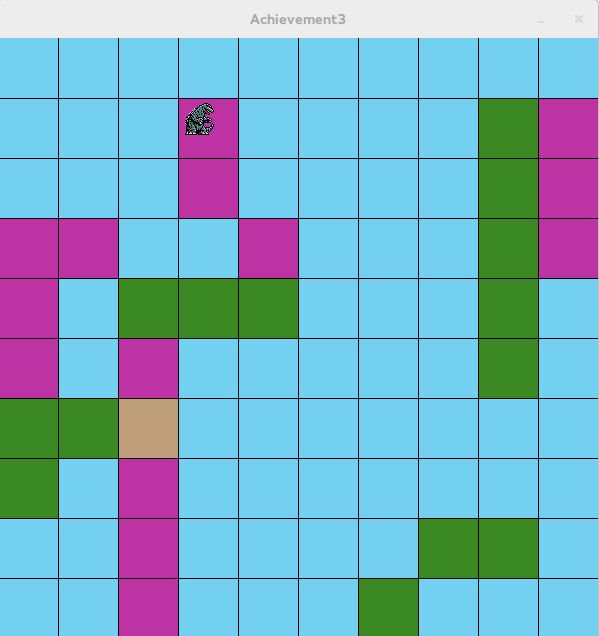
\includegraphics[scale=0.5]{./image/Godzilla_SDL.png}
\end{center}
\newpage
Dans l'affichage en console on va mettre une "*" après la valeur qui se trouve dans la grille comme dans l'exemple en position (9, 8) : \\
\begin{center}
  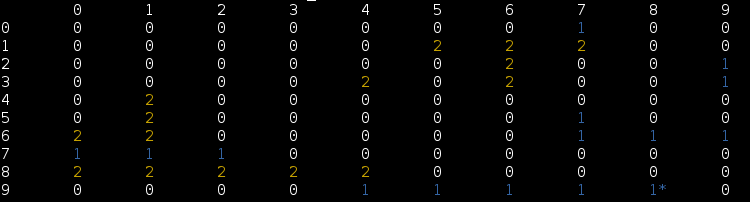
\includegraphics[scale=0.8]{./image/Godzilla_console.png}
\end{center}
\subsection{Fonctionnement de l'achievement3}
Dans notre grille, pour savoir si le monstre est présent, il se trouve à l'indice {\textit{NB\_JOUEURS}} + 1 dans notre tableau de case.\\
Pour réaliser cet achievement on a tout d'abord créer une structure Monstre qui possède :
\begin{itemize}
\item une Position afin de savoir où se trouve le monstre
\item un entier afin de savoir si le monstre a été agressé
\item un tableau d'entier de taille {\textit{NB\_JOUEURS}} pour savoir si le joueur i l'a agressé ou non
\end{itemize}
Puis ensuite il a fallu réaliser les fonctions pour les trois actions différentes qu'il peut réaliser.
\subsubsection{Monstre oblitère des cases}
Cette fonction consiste simplement à oblitérer les cases à gauche, droite, au dessus, en bas, sous le monstre si elles existent et s'il y a un bateau pour cela on utilise la fonction :
\begin{lstlisting}
int monstre_oblitere(struct Grille *grille, struct Monstre *monstre, struct Joueur *j1, struct Joueur *j2);
\end{lstlisting}
Cette fonction renvoie un entier qui correspond au nombre de case que le monstre a oblitéré. Cela nous permet de savoir si le monstre a oblitéré des cases ou si on doit faire l'autre action c'est à dire déplacer le monstre d'une case vers un bateau.\\
La complexité est en $\Theta(n)$ où n est le maximum entre le nombre de case en vie du joueur 1 et 2.
\subsubsection{Déplacement du monstre non agressé}
Cette fonction a pour prototype :
\begin{lstlisting}
void deplacement_monstre_pas_agresse(struct Joueur *j1, struct Joueur *j2, struct Monstre *monstre, struct Grille *grille);
\end{lstlisting}
Pour cette fonction, on a utilisé une fonction auxiliaire qui nous permet de savoir les cases les plus proches d'un monstre :
\begin{lstlisting}
void case_plus_proche_monstre(struct Joueur *j, struct Monstre *monstre, struct Position tab[], int *distance, int *nombre_case);
\end{lstlisting}
Cette fonction consiste à parcourir toutes les cases en vie du joueur et de regarder si la distance est inférieur à celle trouvée avant. Elle est de compléxité $\Theta(n)$ où est le nombre de case en vie du joueur.\\
On doit appliquer cette fonction pour les deux joueurs afin de trouver toutes les cases les plus proches.\\
Ensuite, on choisit une case aléatoire parmi toutes celles possibles et on se déplace d'une case vers elle.\\
La complexité de cette fonction est $\Theta(n + m)$ où n (resp. m) est le nombre de case en vie du joueur 1 (resp. 2). 
\subsubsection{Déplacement du monstre agressé}
Cette fonction a pour prototype :
\begin{lstlisting}
void deplacement_monstre_agresse(struct Grille *grille, struct Monstre *monstre, struct Joueur *j1, struct Joueur *j2, SDL_Surface *ecran, int affichage);
\end{lstlisting}
Premièrement, cette fonction teste si c'est le joueur 1 ou 2 ou les deux qui l'ont agressé afin de savoir vers quel joueur se déplacer. Pour savoir quel est le bateau le plus proche une fois le joueur choisi, on utilise la fonction : 
\begin{lstlisting}
int bateau_le_plus_proche(struct Monstre *monstre,  struct Joueur *j);
\end{lstlisting}
Cette fonction appelle la fonction {\textit{case\_plus\_proche\_monstre}} afin d'avoir la case la plus proche du monstre puis cherche à quel bateau elle appartient. \\
Puis une fois que la fonction {\textit{deplacement\_monstre\_agresse}} renvoie le bateau vers lequel le monstre doit se déplacer, elle fait appel à une fonction auxiliaire qui permet de lister toutes les cases autour des cases en vie du batal et en renvoie une aléatoirement parmi toutes elles. Cette fonction est :
\begin{lstlisting}
struct Position case_autour_du_batal(struct Batal *bat, struct Grille *grille);
\end{lstlisting}
La fonction pour déplacer un monstre agressé est en compléxité $\Theta(n)$ où est le nombre de case qu'occupe tous les batals.
\subsubsection{Tour du monstre}
\begin{lstlisting}
void monstre_qui_joue(struct Monstre *monstre, struct Grille *grille, struct Joueur *joueur1, struct Joueur *joueur2, SDL_Surface *ecran, int affichage){
  if(monstre->agresse)
    deplacement_monstre_agresse(grille, monstre, joueur1, joueur2, ecran, affichage);
  placer_monstre(monstre, grille);
  if(monstre_oblitere(grille, monstre, joueur1, joueur2))
    ;
  else
    deplacement_monstre_pas_agresse(joueur1, joueur2, monstre, grille);
  placer_monstre(monstre, grille);
}
\end{lstlisting}
Premièrement le monstre commence par regarder s'il a été attaqué ou non, si c'est le cas on utilise la fonction {\textit{deplacement\_monstre\_agresse}}. Ensuite, dans tous les cas, on utilise la fonction qui va oblitérer les cases, si elle oblitère des cases, on s'arrête là sinon on va alors appliquer la fonction qui permet de déplacer le monstre lorsqu'il n'est pas agressé.\\
\subsubsection{Affichage du chemin du monstre en SDL}
Pour afficher le chemin on part de la position de départ et on cherche d'abord à ce que le monstre arrive sur la même ligne que sa position d'arrivée. Par exemple si le monstre est en position (8, 2) et doit se rendre en (5, 4) il va se déplacer en (7, 2) puis (6, 2) puis (5, 2). Après on fait la même chose pour les colonnes. Si on reprend notre exemple il va donc aller en (5, 3) puis (5, 4). En SDL, l'affichage se fait comme ceci :
\begin{center}
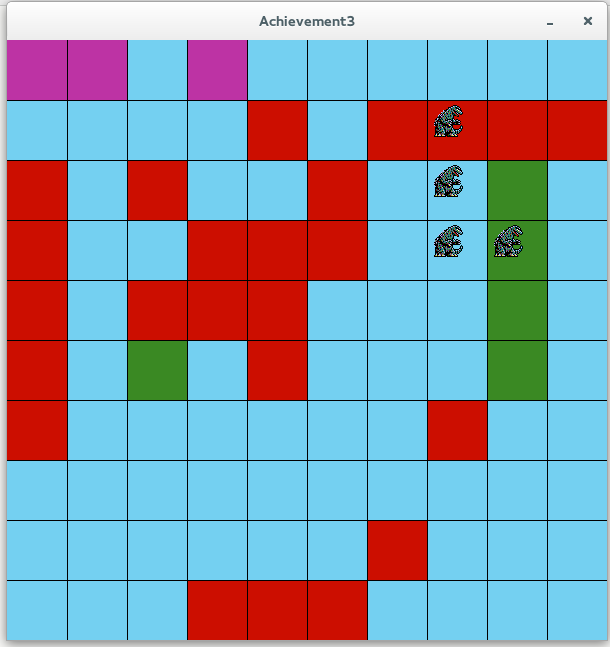
\includegraphics[scale=0.4]{./image/chemin_monstre_SDL}
\end{center}
\subsubsection{Fonctionnement de la boucle de jeu}
Notre fonction qui fait tourner la boucle de jeu a pour prototype :
\begin{lstlisting}
int achievement2(SDL_Surface *ecran, int affichage);
\end{lstlisting}
Elle prend un paramètre un écran si on utilise l'affichage SDL et un entier qui permet de savoir l'affichage souhaité et retourne un entier afin de nous dire le joueur qui a gagné.\\
Notre boucle de jeu tourne tant qu'il reste des bateaux des 2 joueurs et que le nombre de coup n'a pas dépassé la constante {\textit{NB\_COUP\_MAX}}. Dans notre boucle, on va :
\begin{itemize}
\item Déplacer un bateau du joueur1 si c'est possible.
\item Déplacer un bateau du joueur2 si c'est possible.
\item Calculer la position d'arrivée des torpilles pour les deux joueurs.
\item Oblitérer les cases si la position d'arrivée est possible(ie ne dépasse pas la distance maximale)
\item Effectuer le tour du monstre.
\item Incrémenter le nombre de coup
\end{itemize}
La fonction termine pour les mêmes raisons que dans l'achievement1 car notre structure de la boucle reste la même avec juste au début la possibilité de bouger les bateaux et le tour du monstre ce qui ne change pas la valeur de nb\_coup.
\subsection{Problèmes rencontrés}
\begin{itemize}
\item Le premier problème est lorsque le monstre est attaqué par le joueur 1 ou 2, ce n'est pas obligé qu'il puisse trouver un bateau de ce joueur vers lequel aller car il joue après la phase de tir. Comme dans l'exemple, s'il reste une case en vie pour chaque joueur, le joueur 1 attaque le monstre et le joueur2 détruit la dernière case en vie du joueur 1 alors lorsque le tour du monstre vient il ne peut pas se déplacer vers une case en vie du joueur 1 car il n'y en a plus. Donc ceci nous a contraint a modifier notre algorithme pour faire en sorte de ne pas avoir d'erreur si ce cas se produit.\\
\item Au début, on avait oublié d'enlever le monstre de la grille, donc on avait plusieurs monstres sur celle-ci.
\end{itemize}

\newpage
\section{Achievement4}
\subsection{Principe de l’achievement4}

Dans cet achievement, on introduit deux nouveaux objets qui sont les archipals et les portals. Les archipals sont à voir comme des murs infranchissables par les bateaux, les torpilles ou même Godzilla. Les portals sont à voir comme des téléporteurs sur la grille, c'est à dire que quand une case d'un bateau, ou d'une torpille ou de Godzilla arrive sur un portal, elle est téléportée à une autre case associée au portal si elle va dans la direction activé par le portal (un portal téléporte un objet que s'il va dans une direction donnée, vers le haut, le bas, à gauche ou à droite; et cette direction est propre à chaque portal). Ces deux objets entraînent une grande conséquence sur la définition de distance et surtout de distance minimale en ce qui concerne le déplacement des torpilles puisque rappelons que les torpilles doivent aller vers la case d'un batal d'un joueur adverse la plus proche. 

\subsection{Fonctionnement de l'achievement4}

\subsubsection{Les nouvelles structures et constantes}
Pour cet achievement, nous avons besoin de deux nouvelles constantes qui sont:
\begin{itemize}
\item \textit{NB\_PORTALS} est la constante indiquant le nombre de portals que l'on a dans la grille.
\item \textit{NB\_ARCHIPALS} est la constante indiquant le nombre d'archipals que l'on a sur la grille. 
\end{itemize} 
\vspace{0.3cm}
Nous introduisons deux nouvelles structures et une nouvelle énumération:
\begin{itemize}
\item L'énumération \textit{Cote\_case}:
\begin{lstlisting}
enum Cote_case{
  HAUT=1, DROITE, BAS, GAUCHE
};
\end{lstlisting}
Cette énumération est utile pour les portals puisqu'elle va permettre de savoir dans quelle direction aura lieu la téléportation. \\
\item La structure de \textit{Portal}:
\begin{lstlisting}
struct Portal{
  int indpos;
  int arrive;
  enum Cote_case cote;
};
\end{lstlisting}
L'entier \textbf{indpos} est l'indice de la grille où se situe le portal, l'entier \textbf{arrive} est l'indice de la grille où la case sera téléportée lors du passage dans le portal et le \textbf{cote} permet de savoir dans quelle direction s'effectuera la téléportation (HAUT, DROITE, BAS ou GAUCHE).
\newpage
Pour comprendre ce qu'est un portal, regardons l'exemple suivant: \\
\begin{center}
\begin{tabular}[t]{c|c|c|c|c|c|c|c|c|c|c|}
  \multicolumn{1}{c}{} & \multicolumn{1}{c}{0} & \multicolumn{1}{c}{1} & \multicolumn{1}{c}{2} & \multicolumn{1}{c}{3} & \multicolumn{1}{c}{4} & \multicolumn{1}{c}{5} & \multicolumn{1}{c}{6} & \multicolumn{1}{c}{7} & \multicolumn{1}{c}{8} & \multicolumn{1}{c}{9} \\ 
 \cline{2-11} 0 & & & & & & & & & \cellcolor{red} & \\
 \cline{2-11} 1 & & & & & & & & & & \\
 \cline{2-11} 2 & & & & & & & & & & \\
 \cline{2-11} 3 & & & & & & & & & & \\
 \cline{2-11} 4 & & & & & & & & & & \\
 \cline{2-11} 5 & & & & & & & & & & \\
 \cline{2-11} 6 & & & \multicolumn{1}{c||}{\textcolor{red}{8}} & & & & & & & \\
 \cline{2-11} 7 & & & & & & & & & & \\
 \cline{2-11} 8 & & & & & & & & & & \\
 \cline{2-11} 9 & & & & & & & & & & \\
 \cline{2-11} 
\end{tabular} 
\end{center} 
\vspace{0.5cm}
Sur cette exemple, un élément passant sur la case 62 et allant vers la droite se trouvera téléportée sur la case 8 de la grille. \\
\item La structure de \textit{Chemin\_Minimal}:
\begin{lstlisting}
struct Chemin_Minimal{
  int tab[NB_COLONNES*NB_LIGNES];
  int taille;
};
\end{lstlisting}
\end{itemize}
La matrice utile pour l'algorithme de Floyd Warshall sera un tableau linéaire de cette structure, l'entier \textbf{taille} nous permettra de stocker la taille du chemin le plus court et le tableau \textbf{tab} nous permettra de stocker les cases par lesquelles passer pour obtenir le chemin le plus court. 

\subsubsection{L'algorithme de Floyd Warshall}

Pour redéfinir la notion de distance minimale, nous avons décidé d'utiliser l'algorithme de Floyd Warshall en considérant notre grille comme un graphe, chaque case est relié à 4 autres cases (même si c'est un portal) sauf dans le cas où la case est un archipal ou que la case se situe sur une bordure. L'algorithme de Floyd Warshall consiste à comparer deux chemins à chaque fois: le chemin de base (ou chemin le plus court gardé par l'algorithme dans les étapes précédentes) et le chemin en introduisant le passage par un autre sommet, et on garde en mémoire le chemin le plus court pour ensuite recommencer cette comparaison N fois avec N le nombre de sommet dans le graphe. Pour représenter le graphe, nous avons utilisé une matrice de poids où chaque arête est représenté par un poids de 1 dans la matrice initiale, la diagonale est rempli de 0 (arête d'un sommet vers lui même) et les cases inaccessibles d'un sommet à un autre sont représentés par des -1 (il faut voir ces -1 comme représentant l'infini). Il faut savoir que la taille de la matrice est de N*N avec N le nombre de case dans la grille. Comprenons l'algorithme de Floyd Warshall sur un exemple simple:
\begin{center}
$ A^0=
\begin{pmatrix} 
0 & 1 & 1 & 7 \\
-1 & 0 & 1 & 3 \\
-1 & -1 & 0 & 1 \\
-1 & -1 & -1 & 0 \\
\end{pmatrix}
$
\end{center}
Avec cette matrice initiale, on constate que l'on peut aller:
\begin{itemize}
\item du sommet 1 au sommet 2 avec un poids de 1
\item du sommet 1 au sommet 3 avec un poids de 1
\item du sommet 1 au sommet 4 avec un poids de 7
\item du sommet 2 au sommet 3 avec un poids de 1
\item du sommet 2 au sommet 4 avec un poids de 3
\item du sommet 3 au sommet 4 avec un poids de 1
\end{itemize}
Maintenant, on va appliquer la formule de l'algorithme de Floyd Warshall qui est la suivante: 
\begin{center}
$A_{i,j}^k = min ( A_{i,j}^{k-1}, A_{i,k}^{k-1} + A_{k,j}^{k-1} )$ 
\end{center}
Il faut appliquer cette formule pour k allant de 1 à 4 (afin de parcourir tous les sommets).
On obtient donc les matrices suivantes: \\
\begin{center}
$ A^1=
\begin{pmatrix} 
0 & 1 & 1 & 7 \\
-1 & 0 & 1 & 3 \\
-1 & -1 & 0 & 1 \\
-1 & -1 & -1 & 0 \\
\end{pmatrix}
$
$ A^2=
\begin{pmatrix} 
0 & 1 & 1 & \textcolor{red}{4} \\
-1 & 0 & 1 & 3 \\
-1 & -1 & 0 & 1 \\
-1 & -1 & -1 & 0 \\
\end{pmatrix}
$
$ A^3=
\begin{pmatrix} 
0 & 1 & 1 & \textcolor{red}{2} \\
-1 & 0 & 1 & \textcolor{red}{2} \\
-1 & -1 & 0 & 1 \\
-1 & -1 & -1 & 0 \\
\end{pmatrix}
$
\end{center}
Pour au final obtenir la matrice suivante:
\begin{center}
$ A^4=
\begin{pmatrix} 
0 & 1 & 1 & 2 \\
-1 & 0 & 1 & 2 \\
-1 & -1 & 0 & 1 \\
-1 & -1 & -1 & 0 \\
\end{pmatrix}
$
\end{center}
Et maintenant, on peut aller:
\begin{itemize}
\item du sommet 1 au sommet 2 avec un poids de 1
\item du sommet 1 au sommet 3 avec un poids de 1
\item du sommet 1 au sommet 4 avec un poids de 2
\item du sommet 2 au sommet 3 avec un poids de 1
\item du sommet 2 au sommet 4 avec un poids de 2
\item du sommet 3 au sommet 4 avec un poids de 1 \\
\end{itemize}
La fonction qui initialise la matrice est \textit{init\_floyd\_warshall} qui va donc modéliser notre matrice d'adjacence (matrice des poids):
\begin{lstlisting}
void init_floyd_warshall(struct Grille *grille, struct Chemin_Minimal tab[],struct Portal portals[])
\end{lstlisting}
Puis ensuite, on procède à l'algorithme de Floyd Warshall, pour cela nous utilisons la fonction \textit{floyd\_warshall}:
\begin{lstlisting}
void floyd_warshall(struct Chemin_Minimal tab[]) 
\end{lstlisting}
Il faut savoir que l'algorithme de Floyd Warshall a une complexité en temps assez élevée puisqu'elle est en $\Theta(N^{3})$ avec N le nombre de sommet du graphe (ou nombre d'indices dans la matrice de poids). 

\subsubsection{Le fonctionnement général de l'achievement4}
L'achievement4 fonctionne comme l'achievement1 en remplaçant la fonction \textit{distance\_minimale} par la fonction \textit{distminimale} qui utilise la matrice de poids modifiée par l'algorithme de Floyd Warshall.

\subsection{Problèmes rencontrés}

Nous avons rencontrés des problèmes pour cet achievement qui sont les suivants:
\begin{itemize}
\item Le premier problème a été de stocker dans la grille le fait que sur la case on ait un portal ou un archipal, pour les stocker on a donc codé un archipal avec le chiffre $-2$ et on a codé un portal avec l'indice de sa case d'arrivée + 1 (pour pas qu'il y ait de conflit avec la case d'indice 0 puisque le 0 nous sert à identifier l'eau sur la grille). Au moment de l'affichage de la grille, les archipals sont identifiables par des \textcolor{purple}{-2} et les portals par des " ' ".\\
\item Le deuxième problème aura été de choisir entre l'algorithme de Floyd Warshall ou l'algorithme de Dijkstra, puisque l'algorithme de Floyd Warshall a une complexité en temps en $\Theta(N^{3})$ mais on exécute une seule et unique fois l'algorithme sur la matrice, tandis que l'algorithme de Dijkstra est en $\Theta(N^{2})$ mais il faut appliquer l'algorithme à chaque fois que l'on a besoin de la distance minimale entre deux cases (sachant que nous utilisons de nombreuses fois cette fonction), nous aurions pu faire une programmation dynamique aussi avec l'algorithme de Dijkstra, en sauvegardant les distances minimales déjà calculées mais notre choix est resté sur l'algorithme de Floyd Warshall.\\
\item Le troisième problème qui n'a pas été résolu par manque de temps est le déplacement des bateaux dans la grille, puisqu'avec les portals, le déplacement des bateaux devient plus complexe, nous ne pouvons plus assurer la terminaison de notre jeu avec l'algorithme récursif de l'achievement2. 
\end{itemize}

\newpage
\section{Conclusion}
Ce projet nous a permis d'apprendre à travailler en équipe, c'est à dire apprendre à se répartir le travail ainsi qu'à réfléchir à deux avant d'implémenter les choses. C'est un travail formateur pour notre futur métier.\\
Les tests que nous avons effectué lors de tous ces achievements nous ont permis d'éviter de regresser lorsqu'on avançait dans les achievements. Pour un autre projet, une méthode pourrait être de commencer par les tests et ensuite écrire nos fonctions.
\end{document}
